\chapter{El árbol de segmentos, renovado}

\index{{\'a}rbol!de segmentos}

El árbol de segmentos es una estructura de datos versátil que puede
utillizarse para resolver un gran número de problemas algorítmicos. Sin
embargo, hay muchos temas relacionados a los árboles de segmentos que todavía
no hemos visto. Es hora de ver las variantes avanzadas del árbol de
segmentos.

Hasta ahora, hemos implementado las operaciones de un árbol recorriéndolo
\emph{de abajo hacia arriba}. Por ejemplo, hemos calculado sumas en rangos
de la siguiente manera (Capítulo 9.3):

\begin{lstlisting}
int suma(int a, int b) {
    a += n; b += n;
    int s = 0;
    while (a <= b) {
        if (a % 2 == 1) s += árbol[a++];
        if (b % 2 == 0) s += árbol[b--];
        a /= 2; b /= 2;
    }
    return s;
}
\end{lstlisting}

No obstante, en algunos árboles de segmentos más avanzados, a menudo es
necesario implementar las operaciones de otra forma: \emph{de arriba hacia
    abajo}. Usando este método, la función se vuelve:
\begin{lstlisting}
int suma(int a, int b, int k, int x, int y) {
    if (b < x || a > y) return 0;
    if (a <= x && y <= b) return árbol[k];
    int d = (x + y) / 2;
    return suma(a, b, 2 * k, x, d)
         + suma(a, b, 2 * k + 1, d + 1, y);
}
\end{lstlisting}

Ahora podemos calcular cualquier valor de $\texttt{suma}_q(a, b)$---la
suma de valores en el rango $[a,b]$---de la siguiente manera:
\begin{lstlisting}
int s = suma(a, b, 1, 0, n - 1);
\end{lstlisting}

El parámetro $k$ indica la posición actual en el \texttt{árbol}. Inicialmente
$k=1$, porque comenzamos en la raíz del árbol. El rango $[x,y]$ corresponde
a $k$ y es $[0,n-1]$ inicialmente. Cuando calculamos la suma, si $[x,y]$
está fuera de $[a,b]$, la suma es 0, y si $[x,y]$ está completamente dentro
de $[a,b]$, la suma puede encontrarse en el \texttt{árbol}. Si $[x,y]$ está
parcialmente dentro de $[a,b]$, la búsqueda continúa recursivamente a las
mitades izquierda y derecha de $[x,y]$. La mitad izquierda es $[x,d]$ y la
mitad izquierda es $[d+1,y]$ donde $d=\left\lfloor \frac{x+y}{2} \right\rfloor$.

La siguiente imagen muestra cómo la búsqueda procede cuando se calcula el valor
de $\texttt{suma}_q(a,b)$. Los nodos grises indican que la recursión frena
y la suma puede encontrarse en el \texttt{árbol}.

\begin{center}
    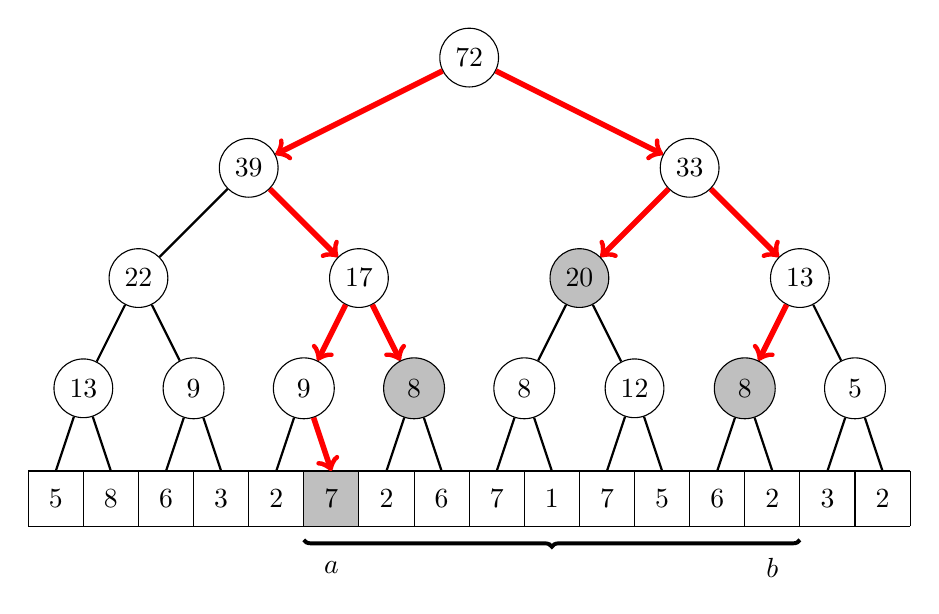
\begin{tikzpicture}[scale=0.7]
        \fill[color=gray!50] (5,0) rectangle (6,1);
        \draw (0,0) grid (16,1);

        \node[anchor=center] at (0.5, 0.5) {5};
        \node[anchor=center] at (1.5, 0.5) {8};
        \node[anchor=center] at (2.5, 0.5) {6};
        \node[anchor=center] at (3.5, 0.5) {3};
        \node[anchor=center] at (4.5, 0.5) {2};
        \node[anchor=center] at (5.5, 0.5) {7};
        \node[anchor=center] at (6.5, 0.5) {2};
        \node[anchor=center] at (7.5, 0.5) {6};
        \node[anchor=center] at (8.5, 0.5) {7};
        \node[anchor=center] at (9.5, 0.5) {1};
        \node[anchor=center] at (10.5, 0.5) {7};
        \node[anchor=center] at (11.5, 0.5) {5};
        \node[anchor=center] at (12.5, 0.5) {6};
        \node[anchor=center] at (13.5, 0.5) {2};
        \node[anchor=center] at (14.5, 0.5) {3};
        \node[anchor=center] at (15.5, 0.5) {2};

        %\node[anchor=center] at (1,2.5) {13};

        \node[draw, circle] (a) at (1,2.5) {13};
        \path[draw,thick,-] (a) -- (0.5,1);
        \path[draw,thick,-] (a) -- (1.5,1);
        \node[draw, circle,minimum size=22pt] (b) at (3,2.5) {9};
        \path[draw,thick,-] (b) -- (2.5,1);
        \path[draw,thick,-] (b) -- (3.5,1);
        \node[draw, circle,minimum size=22pt] (c) at (5,2.5) {9};
        \path[draw,thick,-] (c) -- (4.5,1);
        \path[draw,thick,-] (c) -- (5.5,1);
        \node[draw, circle,fill=gray!50,minimum size=22pt] (d) at (7,2.5) {8};
        \path[draw,thick,-] (d) -- (6.5,1);
        \path[draw,thick,-] (d) -- (7.5,1);
        \node[draw, circle,minimum size=22pt] (e) at (9,2.5) {8};
        \path[draw,thick,-] (e) -- (8.5,1);
        \path[draw,thick,-] (e) -- (9.5,1);
        \node[draw, circle] (f) at (11,2.5) {12};
        \path[draw,thick,-] (f) -- (10.5,1);
        \path[draw,thick,-] (f) -- (11.5,1);
        \node[draw, circle,fill=gray!50,minimum size=22pt] (g) at (13,2.5) {8};
        \path[draw,thick,-] (g) -- (12.5,1);
        \path[draw,thick,-] (g) -- (13.5,1);
        \node[draw, circle,minimum size=22pt] (h) at (15,2.5) {5};
        \path[draw,thick,-] (h) -- (14.5,1);
        \path[draw,thick,-] (h) -- (15.5,1);

        \node[draw, circle] (i) at (2,4.5) {22};
        \path[draw,thick,-] (i) -- (a);
        \path[draw,thick,-] (i) -- (b);
        \node[draw, circle] (j) at (6,4.5) {17};
        \path[draw,thick,-] (j) -- (c);
        \path[draw,thick,-] (j) -- (d);
        \node[draw, circle,fill=gray!50] (k) at (10,4.5) {20};
        \path[draw,thick,-] (k) -- (e);
        \path[draw,thick,-] (k) -- (f);
        \node[draw, circle] (l) at (14,4.5) {13};
        \path[draw,thick,-] (l) -- (g);
        \path[draw,thick,-] (l) -- (h);

        \node[draw, circle] (m) at (4,6.5) {39};
        \path[draw,thick,-] (m) -- (i);
        \path[draw,thick,-] (m) -- (j);
        \node[draw, circle] (n) at (12,6.5) {33};
        \path[draw,thick,-] (n) -- (k);
        \path[draw,thick,-] (n) -- (l);

        \node[draw, circle] (o) at (8,8.5) {72};
        \path[draw,thick,-] (o) -- (m);
        \path[draw,thick,-] (o) -- (n);

        \path[draw=red,thick,->,line width=2pt] (o) -- (m);
        \path[draw=red,thick,->,line width=2pt] (o) -- (n);

        \path[draw=red,thick,->,line width=2pt] (m) -- (j);
        \path[draw=red,thick,->,line width=2pt] (j) -- (c);
        \path[draw=red,thick,->,line width=2pt] (j) -- (d);
        \path[draw=red,thick,->,line width=2pt] (c) -- (5.5,1);

        \path[draw=red,thick,->,line width=2pt] (n) -- (k);
        \path[draw=red,thick,->,line width=2pt] (n) -- (l);

        \path[draw=red,thick,->,line width=2pt] (l) -- (g);

        \draw [decoration={brace}, decorate, line width=0.5mm] (14,-0.25) -- (5,-0.25);

        \node at (5.5,-0.75) {$a$};
        \node at (13.5,-0.75) {$b$};
    \end{tikzpicture}
\end{center}

En esta implementación, las operaciones también tardan $O(\log n)$, porque
el número total de nodos visitados es $O(\log n)$.

\section{Propagación perezosa}

\index{propagación perezosa}
\indexalt{propagación diferida}
\indexalt{lazy propagation}
\index{{\'a}rbol!de segmentos!perezoso}

Usando la \key{propagación perezosa} o \key{diferida}, podemos crear un
árbol de segmentos que soporta tanto actualizaciones como consultas en
rangos, en tiempo $O(\log n)$. La idea es realizar actualizaciones y
consultas de arriba hacia abajo y realizar actualizaciones
\emph{perezosamente}, tal que se propaguen por el árbol hacia abajo
únicamente cuando sea necesario.

En un árbol de segmentos perezoso, los nodos contienen dos tipos de
información. Igual que en un árbol de segmentos ordinario, cada nodo contiene
un valor relacionado al subarreglo correspondiente, como su suma.
Pero además, cada nodo puede contener información relacionada a las
actualizaciones diferidas que no hayan sido propagadas a sus hijos.

Hay dos tipos de actualizaciones en rangos: cada valor es \emph{incrementado}
por un valor o es \emph{asignado} un valor. Ambas operaciones pueden
implementarse utilizando ideas similares, e incluso es posible construir un
árbol que soporte ambas operaciones al mismo tiempo.

\subsubsection{Árboles perezosos}

Considera un ejemplo donde nuestro objetivo es construir un árbol de
segmentos que soporte dos operaciones: incrementar cada valor en $[a,b]$ por
una constante y calcular la suma de valores en $[a,b]$.

Construiremos un árbol donde cada nodo tiene dos valores $s/z$: $s$ denota la
suma de valores en el rango, y $z$ denota el valor de una actualización
perezosa, lo que significa que todos los valores en el rango deben
incrementarse por $z$. En el siguiente árbol, $z=0$ en todos los nodos,
por lo que no hay actualizaciones perezosas en progreso.
\begin{center}
    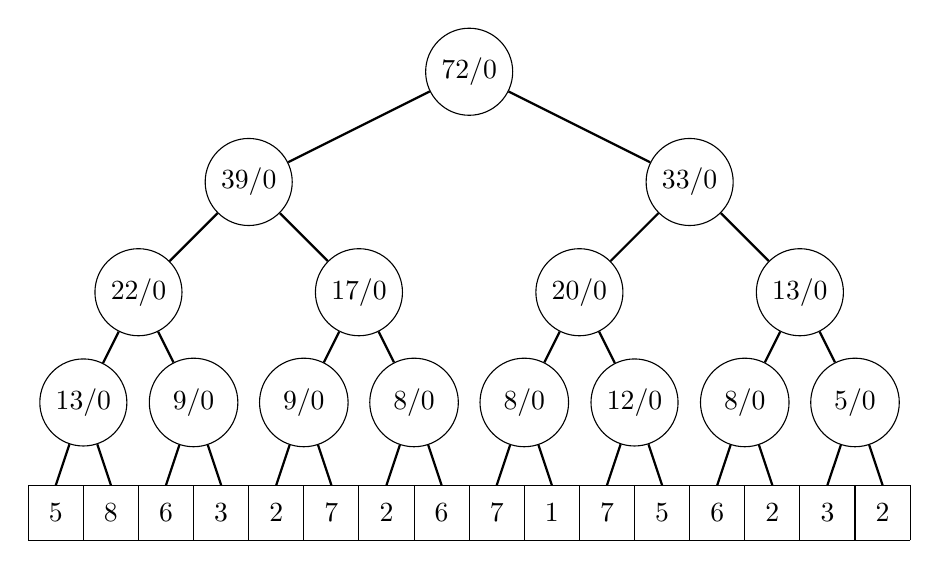
\begin{tikzpicture}[scale=0.7]
        \draw (0,0) grid (16,1);

        \node[anchor=center] at (0.5, 0.5) {5};
        \node[anchor=center] at (1.5, 0.5) {8};
        \node[anchor=center] at (2.5, 0.5) {6};
        \node[anchor=center] at (3.5, 0.5) {3};
        \node[anchor=center] at (4.5, 0.5) {2};
        \node[anchor=center] at (5.5, 0.5) {7};
        \node[anchor=center] at (6.5, 0.5) {2};
        \node[anchor=center] at (7.5, 0.5) {6};
        \node[anchor=center] at (8.5, 0.5) {7};
        \node[anchor=center] at (9.5, 0.5) {1};
        \node[anchor=center] at (10.5, 0.5) {7};
        \node[anchor=center] at (11.5, 0.5) {5};
        \node[anchor=center] at (12.5, 0.5) {6};
        \node[anchor=center] at (13.5, 0.5) {2};
        \node[anchor=center] at (14.5, 0.5) {3};
        \node[anchor=center] at (15.5, 0.5) {2};

        \node[draw, circle] (a) at (1,2.5) {13/0};
        \path[draw,thick,-] (a) -- (0.5,1);
        \path[draw,thick,-] (a) -- (1.5,1);
        \node[draw, circle,minimum size=32pt] (b) at (3,2.5) {9/0};
        \path[draw,thick,-] (b) -- (2.5,1);
        \path[draw,thick,-] (b) -- (3.5,1);
        \node[draw, circle,minimum size=32pt] (c) at (5,2.5) {9/0};
        \path[draw,thick,-] (c) -- (4.5,1);
        \path[draw,thick,-] (c) -- (5.5,1);
        \node[draw, circle,minimum size=32pt] (d) at (7,2.5) {8/0};
        \path[draw,thick,-] (d) -- (6.5,1);
        \path[draw,thick,-] (d) -- (7.5,1);
        \node[draw, circle,minimum size=32pt] (e) at (9,2.5) {8/0};
        \path[draw,thick,-] (e) -- (8.5,1);
        \path[draw,thick,-] (e) -- (9.5,1);
        \node[draw, circle] (f) at (11,2.5) {12/0};
        \path[draw,thick,-] (f) -- (10.5,1);
        \path[draw,thick,-] (f) -- (11.5,1);
        \node[draw, circle,minimum size=32pt] (g) at (13,2.5) {8/0};
        \path[draw,thick,-] (g) -- (12.5,1);
        \path[draw,thick,-] (g) -- (13.5,1);
        \node[draw, circle,minimum size=32pt] (h) at (15,2.5) {5/0};
        \path[draw,thick,-] (h) -- (14.5,1);
        \path[draw,thick,-] (h) -- (15.5,1);

        \node[draw, circle] (i) at (2,4.5) {22/0};
        \path[draw,thick,-] (i) -- (a);
        \path[draw,thick,-] (i) -- (b);
        \node[draw, circle] (j) at (6,4.5) {17/0};
        \path[draw,thick,-] (j) -- (c);
        \path[draw,thick,-] (j) -- (d);
        \node[draw, circle] (k) at (10,4.5) {20/0};
        \path[draw,thick,-] (k) -- (e);
        \path[draw,thick,-] (k) -- (f);
        \node[draw, circle] (l) at (14,4.5) {13/0};
        \path[draw,thick,-] (l) -- (g);
        \path[draw,thick,-] (l) -- (h);

        \node[draw, circle] (m) at (4,6.5) {39/0};
        \path[draw,thick,-] (m) -- (i);
        \path[draw,thick,-] (m) -- (j);
        \node[draw, circle] (n) at (12,6.5) {33/0};
        \path[draw,thick,-] (n) -- (k);
        \path[draw,thick,-] (n) -- (l);

        \node[draw, circle] (o) at (8,8.5) {72/0};
        \path[draw,thick,-] (o) -- (m);
        \path[draw,thick,-] (o) -- (n);
    \end{tikzpicture}
\end{center}

Cuando los elementos en $[a,b]$ se incrementan por $u$, caminamos de la
raíz a las hojas y modificamos los nodos en el árbol de la siguiente
manera: si el rango $[x,y]$ de un nodo se encuentra completamente dentro de
$[a,b]$, incrementamos el valor $z$ del nodo por $u$ y terminamos. Si
$[x,y]$ solo se encuentra parcialmente en $[a,b]$, incrementamos el valor
de $s$ por $hu$, donde $h$ es el tamaño de la intersección de $[a,b]$ y
$[x,y]$, y continuamos nuestra caminata recursivamente en el árbol.

Por ejemplo, la siguiente imagen muestra el árbol luego de incrementar los
elementos en $[a,b]$ por 2:
\begin{center}
    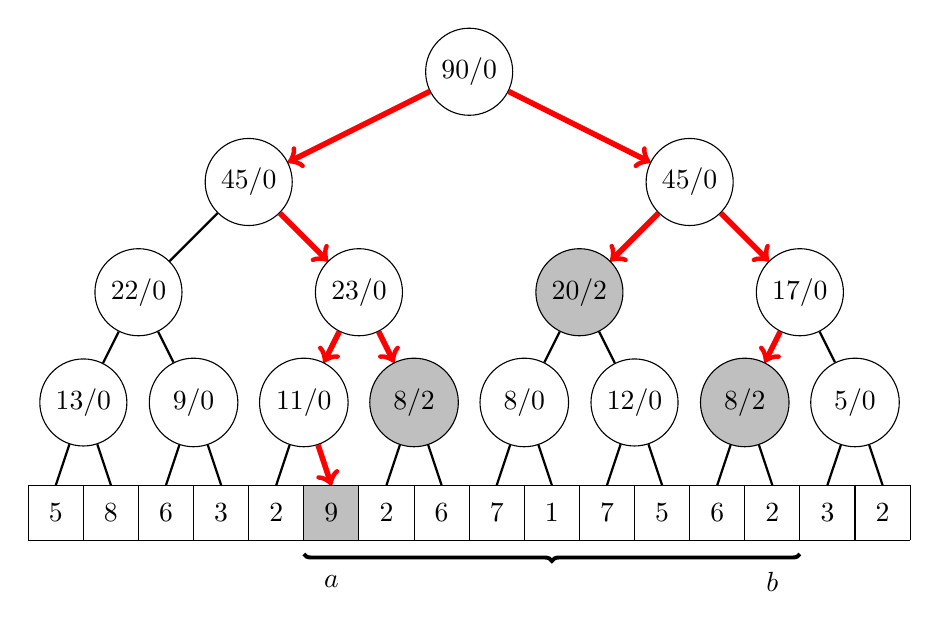
\begin{tikzpicture}[scale=0.7]
        \fill[color=gray!50] (5,0) rectangle (6,1);
        \draw (0,0) grid (16,1);

        \node[anchor=center] at (0.5, 0.5) {5};
        \node[anchor=center] at (1.5, 0.5) {8};
        \node[anchor=center] at (2.5, 0.5) {6};
        \node[anchor=center] at (3.5, 0.5) {3};
        \node[anchor=center] at (4.5, 0.5) {2};
        \node[anchor=center] at (5.5, 0.5) {9};
        \node[anchor=center] at (6.5, 0.5) {2};
        \node[anchor=center] at (7.5, 0.5) {6};
        \node[anchor=center] at (8.5, 0.5) {7};
        \node[anchor=center] at (9.5, 0.5) {1};
        \node[anchor=center] at (10.5, 0.5) {7};
        \node[anchor=center] at (11.5, 0.5) {5};
        \node[anchor=center] at (12.5, 0.5) {6};
        \node[anchor=center] at (13.5, 0.5) {2};
        \node[anchor=center] at (14.5, 0.5) {3};
        \node[anchor=center] at (15.5, 0.5) {2};

        \node[draw, circle] (a) at (1,2.5) {13/0};
        \path[draw,thick,-] (a) -- (0.5,1);
        \path[draw,thick,-] (a) -- (1.5,1);
        \node[draw, circle,minimum size=32pt] (b) at (3,2.5) {9/0};
        \path[draw,thick,-] (b) -- (2.5,1);
        \path[draw,thick,-] (b) -- (3.5,1);
        \node[draw, circle,minimum size=32pt] (c) at (5,2.5) {11/0};
        \path[draw,thick,-] (c) -- (4.5,1);
        \path[draw,thick,-] (c) -- (5.5,1);
        \node[draw, circle,fill=gray!50,minimum size=32pt] (d) at (7,2.5) {8/2};
        \path[draw,thick,-] (d) -- (6.5,1);
        \path[draw,thick,-] (d) -- (7.5,1);
        \node[draw, circle,minimum size=32pt] (e) at (9,2.5) {8/0};
        \path[draw,thick,-] (e) -- (8.5,1);
        \path[draw,thick,-] (e) -- (9.5,1);
        \node[draw, circle] (f) at (11,2.5) {12/0};
        \path[draw,thick,-] (f) -- (10.5,1);
        \path[draw,thick,-] (f) -- (11.5,1);
        \node[draw, circle,fill=gray!50,minimum size=32pt] (g) at (13,2.5) {8/2};
        \path[draw,thick,-] (g) -- (12.5,1);
        \path[draw,thick,-] (g) -- (13.5,1);
        \node[draw, circle,minimum size=32pt] (h) at (15,2.5) {5/0};
        \path[draw,thick,-] (h) -- (14.5,1);
        \path[draw,thick,-] (h) -- (15.5,1);

        \node[draw, circle] (i) at (2,4.5) {22/0};
        \path[draw,thick,-] (i) -- (a);
        \path[draw,thick,-] (i) -- (b);
        \node[draw, circle] (j) at (6,4.5) {23/0};
        \path[draw,thick,-] (j) -- (c);
        \path[draw,thick,-] (j) -- (d);
        \node[draw, circle,fill=gray!50] (k) at (10,4.5) {20/2};
        \path[draw,thick,-] (k) -- (e);
        \path[draw,thick,-] (k) -- (f);
        \node[draw, circle] (l) at (14,4.5) {17/0};
        \path[draw,thick,-] (l) -- (g);
        \path[draw,thick,-] (l) -- (h);

        \node[draw, circle] (m) at (4,6.5) {45/0};
        \path[draw,thick,-] (m) -- (i);
        \path[draw,thick,-] (m) -- (j);
        \node[draw, circle] (n) at (12,6.5) {45/0};
        \path[draw,thick,-] (n) -- (k);
        \path[draw,thick,-] (n) -- (l);

        \node[draw, circle] (o) at (8,8.5) {90/0};
        \path[draw,thick,-] (o) -- (m);
        \path[draw,thick,-] (o) -- (n);

        \path[draw=red,thick,->,line width=2pt] (o) -- (m);
        \path[draw=red,thick,->,line width=2pt] (o) -- (n);

        \path[draw=red,thick,->,line width=2pt] (m) -- (j);
        \path[draw=red,thick,->,line width=2pt] (j) -- (c);
        \path[draw=red,thick,->,line width=2pt] (j) -- (d);
        \path[draw=red,thick,->,line width=2pt] (c) -- (5.5,1);

        \path[draw=red,thick,->,line width=2pt] (n) -- (k);
        \path[draw=red,thick,->,line width=2pt] (n) -- (l);

        \path[draw=red,thick,->,line width=2pt] (l) -- (g);

        \draw [decoration={brace}, decorate, line width=0.5mm] (14,-0.25) -- (5,-0.25);

        \node at (5.5,-0.75) {$a$};
        \node at (13.5,-0.75) {$b$};
    \end{tikzpicture}
\end{center}

Ahora también calculamos la suma de elementos en el rango $[a,b]$ caminando
en el árbol de arriba hacia abajo. Si el rango $[x,y]$ de un nodo pertenece
completamente a $[a,b]$, añadimos el valor $s$ del nodo a la suma. De lo
contrario, continuamos la búsqueda recursivamente a través del árbol.

Tanto en actualizaciones como en consultas, el valor de una actualización
perezosa siempre es propagado a los hijos del nodo antes de procesarlo. La
idea es que las actualizaciones se propaguen solo cuando sea necesario, lo
que garantiza que las operaciones siempre son eficientes.

La siguiente imagen muestra cómo cambia el árbol cuando calculamos el valor
de $\texttt{suma}_q(a,b)$. El rectángulo muestra los nodos cuyos valores
cambian, porque una actualización perezosa se propaga hacia abajo.

\begin{center}
    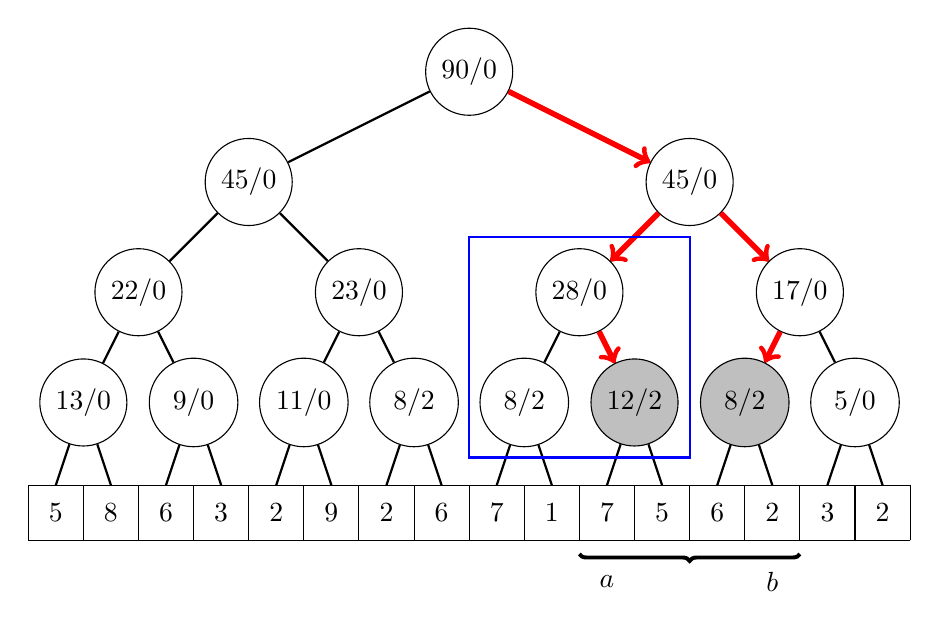
\begin{tikzpicture}[scale=0.7]
        \draw (0,0) grid (16,1);

        \node[anchor=center] at (0.5, 0.5) {5};
        \node[anchor=center] at (1.5, 0.5) {8};
        \node[anchor=center] at (2.5, 0.5) {6};
        \node[anchor=center] at (3.5, 0.5) {3};
        \node[anchor=center] at (4.5, 0.5) {2};
        \node[anchor=center] at (5.5, 0.5) {9};
        \node[anchor=center] at (6.5, 0.5) {2};
        \node[anchor=center] at (7.5, 0.5) {6};
        \node[anchor=center] at (8.5, 0.5) {7};
        \node[anchor=center] at (9.5, 0.5) {1};
        \node[anchor=center] at (10.5, 0.5) {7};
        \node[anchor=center] at (11.5, 0.5) {5};
        \node[anchor=center] at (12.5, 0.5) {6};
        \node[anchor=center] at (13.5, 0.5) {2};
        \node[anchor=center] at (14.5, 0.5) {3};
        \node[anchor=center] at (15.5, 0.5) {2};

        \node[draw, circle] (a) at (1,2.5) {13/0};
        \path[draw,thick,-] (a) -- (0.5,1);
        \path[draw,thick,-] (a) -- (1.5,1);
        \node[draw, circle,minimum size=32pt] (b) at (3,2.5) {9/0};
        \path[draw,thick,-] (b) -- (2.5,1);
        \path[draw,thick,-] (b) -- (3.5,1);
        \node[draw, circle,minimum size=32pt] (c) at (5,2.5) {11/0};
        \path[draw,thick,-] (c) -- (4.5,1);
        \path[draw,thick,-] (c) -- (5.5,1);
        \node[draw, circle,minimum size=32pt] (d) at (7,2.5) {8/2};
        \path[draw,thick,-] (d) -- (6.5,1);
        \path[draw,thick,-] (d) -- (7.5,1);
        \node[draw, circle,minimum size=32pt] (e) at (9,2.5) {8/2};
        \path[draw,thick,-] (e) -- (8.5,1);
        \path[draw,thick,-] (e) -- (9.5,1);
        \node[draw, circle,fill=gray!50,] (f) at (11,2.5) {12/2};
        \path[draw,thick,-] (f) -- (10.5,1);
        \path[draw,thick,-] (f) -- (11.5,1);
        \node[draw, circle,fill=gray!50,minimum size=32pt] (g) at (13,2.5) {8/2};
        \path[draw,thick,-] (g) -- (12.5,1);
        \path[draw,thick,-] (g) -- (13.5,1);
        \node[draw, circle,minimum size=32pt] (h) at (15,2.5) {5/0};
        \path[draw,thick,-] (h) -- (14.5,1);
        \path[draw,thick,-] (h) -- (15.5,1);

        \node[draw, circle] (i) at (2,4.5) {22/0};
        \path[draw,thick,-] (i) -- (a);
        \path[draw,thick,-] (i) -- (b);
        \node[draw, circle] (j) at (6,4.5) {23/0};
        \path[draw,thick,-] (j) -- (c);
        \path[draw,thick,-] (j) -- (d);
        \node[draw, circle] (k) at (10,4.5) {28/0};
        \path[draw,thick,-] (k) -- (e);
        \path[draw,thick,-] (k) -- (f);
        \node[draw, circle] (l) at (14,4.5) {17/0};
        \path[draw,thick,-] (l) -- (g);
        \path[draw,thick,-] (l) -- (h);

        \node[draw, circle] (m) at (4,6.5) {45/0};
        \path[draw,thick,-] (m) -- (i);
        \path[draw,thick,-] (m) -- (j);
        \node[draw, circle] (n) at (12,6.5) {45/0};
        \path[draw,thick,-] (n) -- (k);
        \path[draw,thick,-] (n) -- (l);

        \node[draw, circle] (o) at (8,8.5) {90/0};
        \path[draw,thick,-] (o) -- (m);
        \path[draw,thick,-] (o) -- (n);

        \path[draw=red,thick,->,line width=2pt] (o) -- (n);

        \path[draw=red,thick,->,line width=2pt] (n) -- (k);
        \path[draw=red,thick,->,line width=2pt] (n) -- (l);

        \path[draw=red,thick,->,line width=2pt] (k) -- (f);
        \path[draw=red,thick,->,line width=2pt] (l) -- (g);

        \draw [decoration={brace}, decorate, line width=0.5mm] (14,-0.25) -- (10,-0.25);

        \draw[color=blue,thick] (8,1.5) rectangle (12,5.5);

        \node at (10.5,-0.75) {$a$};
        \node at (13.5,-0.75) {$b$};
    \end{tikzpicture}
\end{center}

Ten en cuenta que a veces es necesario combinar actualizaciones perezosas.
Esto sucede cuando un nodo que ya tiene una actualización pendiente es
asignado otra. Cuando calculamos sumas, es fácil combinar actualizaciones
porque la combinación de dos actualizaciones $z_1$ y $z_2$ corresponde a
una tercera $z_1+z_2$.

\subsubsection{Actualizaciones polinómicas}

Las actualizaciones perezosas pueden generalizarse tal que sea posible
actualizar rangos usando polinomios en la forma
\[p(u) = t_k u^k + t_{k-1} u^{k-1} + \cdots + t_0.\]

En este caso, la actualización de un valor en la posición $i$ en $[a,b]$
es $p(i-a)$. Por ejemplo, añadir el polinomio $p(u)=u+1$ a $[a,b]$ significa
que el valor en la posición $a$ se aumenta por 1, aquel en $a+1$ por 2,
y así sucesivamente.

Para soportar actualizaciones polinómicas, cada nodo es asignado $k+2$
valores, donde $k$ es igual al grado del polinomio. El valor $s$ es la suma
de los elementos en el rango, y los valores $z_0,z_1,\ldots,z_k$ son los
coeficientes de un polinomio que corresponde a una actualización perezosa.

Ahora, la suma de valores en un rango $[x,y]$ equivale a
\[s+\sum_{u=0}^{y-x} z_k u^k + z_{k-1} u^{k-1} + \cdots + z_0.\]

El valor de una suma tal puede calcularse eficientemente usando fórmulas de
sumatoria. Por ejemplo, el término $z_0$ corresponde a la suma $(y-x+1)z_0$,
y el término $z_1 u$ corresponde a la suma
\[z_1(0+1+\cdots+y-x) = z_1 \frac{(y-x)(y-x+1)}{2} .\]

Cuando se propaga una actualización en el árbol, los índices de $p(u)$
cambian, porque en cada rango $[x,y]$, los valores se calculan para
$u=0,1,\ldots,y-x$. Sin embargo, esto no causa problemas porque
$p'(u)=p(u+h)$ es un polinomio de grado igual a $p(u)$. Por ejemplo, si
$p(u)=t_2 u^2+t_1 u-t_0$, entonces
\[p'(u)=t_2(u+h)^2+t_1(u+h)-t_0=t_2 u^2 + (2ht_2+t_1)u+t_2h^2+t_1h-t_0.\]

\section{Árboles dinámicos}

\index{{\'a}rbol!de segmentos!din{\'a}mico}

Un árbol de segmentos ordinario es estático, lo que significa que cada nodo
tiene una posición fija en el arreglo y el árbol requiere una cantidad fija
de memoria. En un \key{árbol de segmentos dinámico}, la memoria se asigna
solamente para los nodos que realmente se acceden durante el algoritmo, lo
que puede ahorrar una gran cantidad de memoria.

Los nodos de un árbol dinámico pueden ser representados como \texttt{struct}s:
\begin{lstlisting}
struct nodo {
    int valor;
    int x, y;
    nodo *izquierda, *derecha;
    nodo(int v, int x, int y) : valor(v), x(x), y(y) {}
};
\end{lstlisting}
Aquí, \texttt{valor} es el valor del nodo, $[\texttt{x},\texttt{y}]$ es el
rango correspondiente, e \texttt{izquierda} y \texttt{derecha} apuntan a los
subárboles izquierdo y derecho.

Luego de esto, podemos crear nodos de la siguiente manera:
\begin{lstlisting}
// crear nuevo nodo
nodo *x = new nodo(0, 0, 15);
// modificar valor
x->valor = 5;
\end{lstlisting}

\subsubsection{Árboles de segmentos dispersos}

\index{{\'a}rbol!de segmentos!disperso}

Un árbol de segmentos dinámico es útil cuando el arreglo subyacente es
\emph{disperso}, o sea, el rango $[0,n-1]$ de índices permitidos es grande,
pero la mayoría de los valores son cero. Mientras que un árbol de segmentos
ordinario usa $O(n)$ de memoria, un árbol dinámico solo utiliza $O(k \log n)$,
donde $k$ es el número de operaciones realizadas.

Un \key{árbol de segmentos disperso} inicialmente solo contiene un nodo
$[0,n-1]$ cuyo valor es cero, lo que significa que cada valor del arreglo es
cero. Luego de una actualización, se añaden nuevos nodos dinámicamente al
árbol. Por ejemplo, si $n=16$ y los elementos en las posiciones 3 y 10 fueron
modificados, el nuevo árbol contiene los siguientes nodos:
\begin{center}
    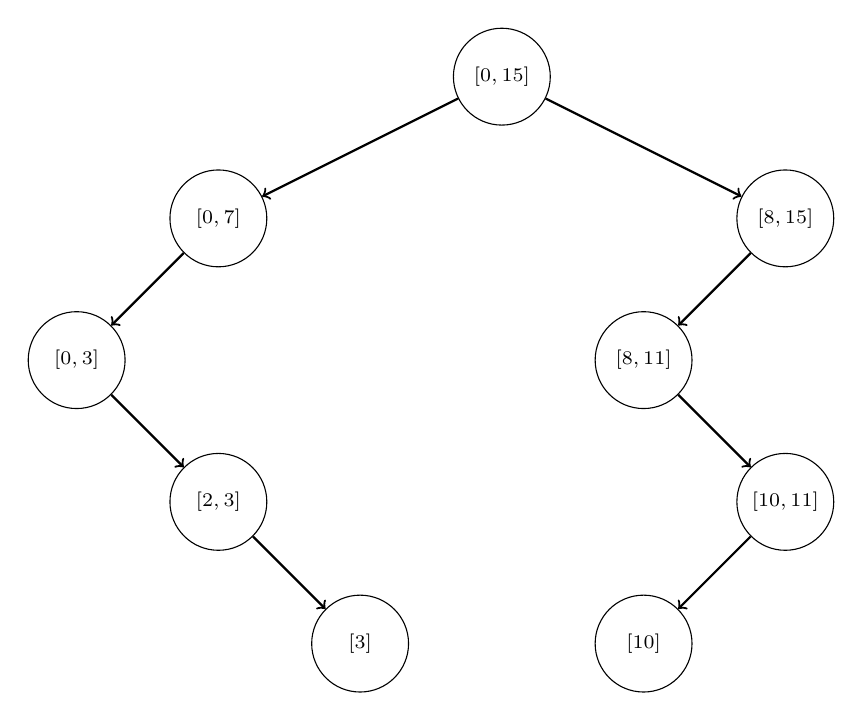
\begin{tikzpicture}[scale=0.9]
        \scriptsize
        \node[draw, circle,minimum size=35pt] (1) at (0,0) {$[0,15]$};
        \node[draw, circle,minimum size=35pt] (2) at (-4,-2) {$[0,7]$};
        \node[draw, circle,minimum size=35pt] (3) at (-6,-4) {$[0,3]$};
        \node[draw, circle,minimum size=35pt] (4) at (-4,-6) {$[2,3]$};
        \node[draw, circle,minimum size=35pt] (5) at (-2,-8) {$[3]$};
        \node[draw, circle,minimum size=35pt] (6) at (4,-2) {$[8,15]$};
        \node[draw, circle,minimum size=35pt] (7) at (2,-4) {$[8,11]$};
        \node[draw, circle,minimum size=35pt] (8) at (4,-6) {$[10,11]$};
        \node[draw, circle,minimum size=35pt] (9) at (2,-8) {$[10]$};

        \path[draw,thick,->] (1) -- (2);
        \path[draw,thick,->] (2) -- (3);
        \path[draw,thick,->] (3) -- (4);
        \path[draw,thick,->] (4) -- (5);

        \path[draw,thick,->] (1) -- (6);
        \path[draw,thick,->] (6) -- (7);
        \path[draw,thick,->] (7) -- (8);
        \path[draw,thick,->] (8) -- (9);
    \end{tikzpicture}
\end{center}

Cualquier camino de la raíz a una hoja contiene $O(\log n)$ nodos, por lo que
cada operación añade como mucho $O(\log n)$ nodos nuevos al árbol. Por ende,
luego de $k$ operaciones, el árbol contiene como mucho $O(k \log n)$ nodos.

Observa que si conocemos todos los elementos que serán actualizados al
comienzo del algoritmo, un árbol de segmentos dinámico no es necesario,
porque podemos usar un árbol de segmentos ordinario con la ayuda de la
compresión de índices (Capítulo 9.4). Esto no es posible cuando los índices
se generan durante la ejecución del algoritmo.

\subsubsection{Árboles de segmentos persistentes}

\index{{\'a}rbol!de segmentos!persistente}

Utilizando una implementación dinámica, también es posible crear un
\key{árbol de segmentos persistente} que almacena la \emph{historia
    de modificaciones} del árbol. En una implementación de estas, podemos,
eficientemente, acceder todas las versiones del árbol que han existido
durante la ejecución del algoritmo.

Cuando esta historia está disponible, podemos realizar consultas en cualquier
árbol previo tal como en un árbol de segmentos ordinario, porque la
estructura completa de cada árbol es almacenada. También podemos crear nuevos
árboles basados en versiones previas y modificarlos independientemente.

\pagebreak
Considera la siguiente secuencia de actualizaciones, donde los nodos rojos
cambian y el resto se mantiene igual:

\begin{center}
    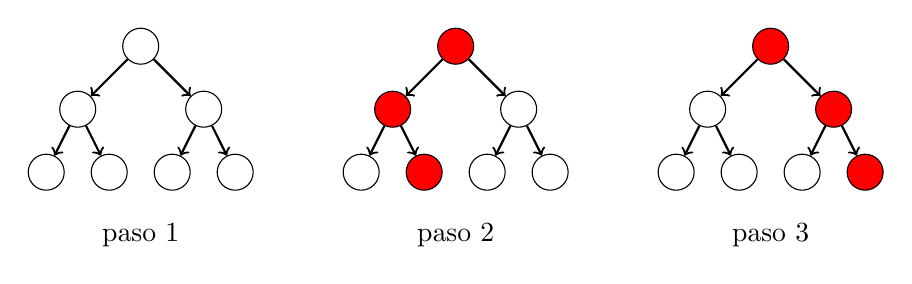
\begin{tikzpicture}[scale=0.8]
        \node[draw, circle,minimum size=13pt] (1a) at (3,0) {};
        \node[draw, circle,minimum size=13pt] (2a) at (2,-1) {};
        \node[draw, circle,minimum size=13pt] (3a) at (4,-1) {};
        \node[draw, circle,minimum size=13pt] (4a) at (1.5,-2) {};
        \node[draw, circle,minimum size=13pt] (5a) at (2.5,-2) {};
        \node[draw, circle,minimum size=13pt] (6a) at (3.5,-2) {};
        \node[draw, circle,minimum size=13pt] (7a) at (4.5,-2) {};
        \path[draw,thick,->] (1a) -- (2a);
        \path[draw,thick,->] (1a) -- (3a);
        \path[draw,thick,->] (2a) -- (4a);
        \path[draw,thick,->] (2a) -- (5a);
        \path[draw,thick,->] (3a) -- (6a);
        \path[draw,thick,->] (3a) -- (7a);

        \node[draw, circle,minimum size=13pt,fill=red] (1b) at (3+5,0) {};
        \node[draw, circle,minimum size=13pt,fill=red] (2b) at (2+5,-1) {};
        \node[draw, circle,minimum size=13pt] (3b) at (4+5,-1) {};
        \node[draw, circle,minimum size=13pt] (4b) at (1.5+5,-2) {};
        \node[draw, circle,minimum size=13pt,fill=red] (5b) at (2.5+5,-2) {};
        \node[draw, circle,minimum size=13pt] (6b) at (3.5+5,-2) {};
        \node[draw, circle,minimum size=13pt] (7b) at (4.5+5,-2) {};
        \path[draw,thick,->] (1b) -- (2b);
        \path[draw,thick,->] (1b) -- (3b);
        \path[draw,thick,->] (2b) -- (4b);
        \path[draw,thick,->] (2b) -- (5b);
        \path[draw,thick,->] (3b) -- (6b);
        \path[draw,thick,->] (3b) -- (7b);

        \node[draw, circle,minimum size=13pt,fill=red] (1c) at (3+10,0) {};
        \node[draw, circle,minimum size=13pt] (2c) at (2+10,-1) {};
        \node[draw, circle,minimum size=13pt,fill=red] (3c) at (4+10,-1) {};
        \node[draw, circle,minimum size=13pt] (4c) at (1.5+10,-2) {};
        \node[draw, circle,minimum size=13pt] (5c) at (2.5+10,-2) {};
        \node[draw, circle,minimum size=13pt] (6c) at (3.5+10,-2) {};
        \node[draw, circle,minimum size=13pt,fill=red] (7c) at (4.5+10,-2) {};
        \path[draw,thick,->] (1c) -- (2c);
        \path[draw,thick,->] (1c) -- (3c);
        \path[draw,thick,->] (2c) -- (4c);
        \path[draw,thick,->] (2c) -- (5c);
        \path[draw,thick,->] (3c) -- (6c);
        \path[draw,thick,->] (3c) -- (7c);

        \node at (3,-3) {paso 1};
        \node at (3+5,-3) {paso 2};
        \node at (3+10,-3) {paso 3};
    \end{tikzpicture}
\end{center}

Tras cada actualización, la mayoría de los nodos se mantienen iguales,
por lo que una forma eficiente de almacenar la historia es representando
cada árbol previo como una combinación de nodos nuevos y subárboles de
árboles anteriores. En este ejemplo, podemos almacenar la historia así:
\begin{center}
    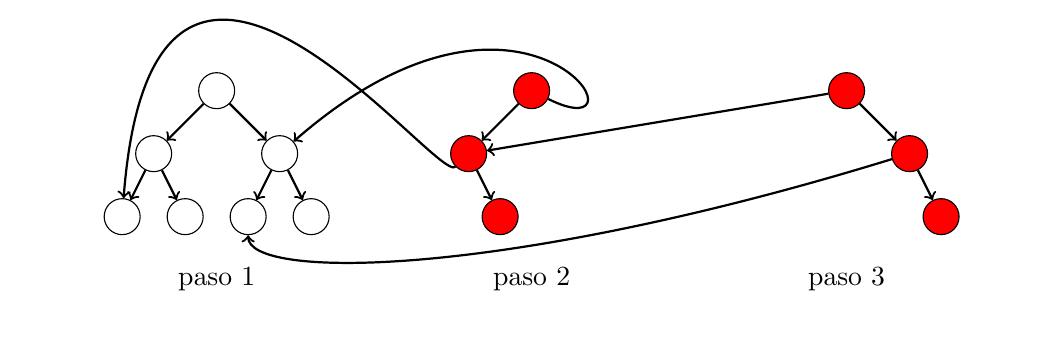
\begin{tikzpicture}[scale=0.8]
        \path[use as bounding box] (0, 1) rectangle (16, -3.5);

        \node[draw, circle,minimum size=13pt] (1a) at (3,0) {};
        \node[draw, circle,minimum size=13pt] (2a) at (2,-1) {};
        \node[draw, circle,minimum size=13pt] (3a) at (4,-1) {};
        \node[draw, circle,minimum size=13pt] (4a) at (1.5,-2) {};
        \node[draw, circle,minimum size=13pt] (5a) at (2.5,-2) {};
        \node[draw, circle,minimum size=13pt] (6a) at (3.5,-2) {};
        \node[draw, circle,minimum size=13pt] (7a) at (4.5,-2) {};
        \path[draw,thick,->] (1a) -- (2a);
        \path[draw,thick,->] (1a) -- (3a);
        \path[draw,thick,->] (2a) -- (4a);
        \path[draw,thick,->] (2a) -- (5a);
        \path[draw,thick,->] (3a) -- (6a);
        \path[draw,thick,->] (3a) -- (7a);

        \node[draw, circle,minimum size=13pt,fill=red] (1b) at (3+5,0) {};
        \node[draw, circle,minimum size=13pt,fill=red] (2b) at (2+5,-1) {};
        \node[draw, circle,minimum size=13pt,fill=red] (5b) at (2.5+5,-2) {};
        \path[draw,thick,->] (1b) -- (2b);

        \draw[thick,->] (1b) .. controls (3+5+2,0-1) and (3+5,2.5) .. (3a);

        \draw[thick,->] (2b) .. controls (2+5-0.5,-1-0.5) and (2,4.5) .. (4a);


        \path[draw,thick,->] (2b) -- (5b);

        \node[draw, circle,minimum size=13pt,fill=red] (1c) at (3+10,0) {};
        \node[draw, circle,minimum size=13pt,fill=red] (3c) at (4+10,-1) {};
        \node[draw, circle,minimum size=13pt,fill=red] (7c) at (4.5+10,-2) {};
        \path[draw,thick,->] (1c) -- (2b);
        \path[draw,thick,->] (1c) -- (3c);

        \draw[thick,->] (3c) .. controls (2.5+5,-3) and (3.5,-3) .. (6a);

        \path[draw,thick,->] (3c) -- (7c);

        \node at (3,-3) {paso 1};
        \node at (3+5,-3) {paso 2};
        \node at (3+10,-3) {paso 3};
    \end{tikzpicture}
\end{center}

Podemos reconstruir la estructura de cada árbol previo siguiende los
punteros, comenzando en la raíz correspondiente. Ya que cada operación
solo añade $O(\log n)$ nodos al árbol, es posible almacenar la historia
completa del árbol.

\section{Estructuras de datos}

En vez de valores individuales, los nodos en un árbol de segmentos también
pueden contener \emph{estructuras de datos} que mantienen información sobre
los rangos correspondientes. En un árbol de estos, las operaciones tadan
$O(f(n) \log n)$, donde $f(n)$ es el tiempo necesario para procesar un
solo nodo durante una operación.

Por ejemplo, considera un árbol de segmentos que soporta consultas del tipo
``¿cuántas veces aparece un elemento $x$ en el rango $[a,b]$?'' Por ejemplo
el elemento 1 aparece tres veces en el siguiente rango:

\begin{center}
    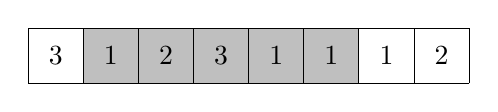
\begin{tikzpicture}[scale=0.7]
        \fill[lightgray] (1,0) rectangle (6,1);
        \draw (0,0) grid (8,1);

        \node[anchor=center] at (0.5, 0.5) {3};
        \node[anchor=center] at (1.5, 0.5) {1};
        \node[anchor=center] at (2.5, 0.5) {2};
        \node[anchor=center] at (3.5, 0.5) {3};
        \node[anchor=center] at (4.5, 0.5) {1};
        \node[anchor=center] at (5.5, 0.5) {1};
        \node[anchor=center] at (6.5, 0.5) {1};
        \node[anchor=center] at (7.5, 0.5) {2};
    \end{tikzpicture}
\end{center}

Para permitir estas consultas, construimos un árbol de segmentos donde
cada nodo es asignado una estructura de datos que puede calcular cuantas
veces un elemento $x$ aparece en el rango correspondiente. Usando este árbol,
la respuesta a una consulta puede calcularse combinando los resultados de
los nodos que pertenecen al rango.

\pagebreak
Por ejemplo, el siguiente árbol de segmentos corresponde al arreglo anterior:
\begin{center}
    \begin{tikzpicture}[scale=1]

        \node[draw, rectangle] (a) at (1,2.5)
        {
            \footnotesize
            \begin{tabular}{r}
                3 \\
                \hline
                1 \\
            \end{tabular}};
        \node[draw, rectangle] (b) at (3,2.5)
        {
            \footnotesize
            \begin{tabular}{r}
                1 \\
                \hline
                1 \\
            \end{tabular}};
        \node[draw, rectangle] (c) at (5,2.5)
        {
            \footnotesize
            \begin{tabular}{r}
                2 \\
                \hline
                1 \\
            \end{tabular}};
        \node[draw, rectangle] (d) at (7,2.5)
        {
            \footnotesize
            \begin{tabular}{r}
                3 \\
                \hline
                1 \\
            \end{tabular}};
        \node[draw, rectangle] (e) at (9,2.5)
        {
            \footnotesize
            \begin{tabular}{r}
                1 \\
                \hline
                1 \\
            \end{tabular}};
        \node[draw, rectangle] (f) at (11,2.5)
        {
            \footnotesize
            \begin{tabular}{r}
                1 \\
                \hline
                1 \\
            \end{tabular}};
        \node[draw, rectangle] (g) at (13,2.5)
        {
            \footnotesize
            \begin{tabular}{r}
                1 \\
                \hline
                1 \\
            \end{tabular}};
        \node[draw, rectangle] (h) at (15,2.5)
        {
            \footnotesize
            \begin{tabular}{r}
                2 \\
                \hline
                1 \\
            \end{tabular}};

        \node[draw, rectangle] (i) at (2,4.5)
        {
            \footnotesize
            \begin{tabular}{rr}
                1 & 3 \\
                \hline
                1 & 1 \\
            \end{tabular}};
        \path[draw,thick,-] (i) -- (a);
        \path[draw,thick,-] (i) -- (b);
        \node[draw, rectangle] (j) at (6,4.5)
        {
            \footnotesize
            \begin{tabular}{rr}
                2 & 3 \\
                \hline
                1 & 1 \\
            \end{tabular}};
        \path[draw,thick,-] (j) -- (c);
        \path[draw,thick,-] (j) -- (d);
        \node[draw, rectangle] (k) at (10,4.5)
        {
            \footnotesize
            \begin{tabular}{r}
                1 \\
                \hline
                2 \\
            \end{tabular}};
        \path[draw,thick,-] (k) -- (e);
        \path[draw,thick,-] (k) -- (f);
        \node[draw, rectangle] (l) at (14,4.5)
        {
            \footnotesize
            \begin{tabular}{rr}
                1 & 2 \\
                \hline
                1 & 1 \\
            \end{tabular}};
        \path[draw,thick,-] (l) -- (g);
        \path[draw,thick,-] (l) -- (h);

        \node[draw, rectangle] (m) at (4,6.5)
        {
            \footnotesize
            \begin{tabular}{rrr}
                1 & 2 & 3 \\
                \hline
                1 & 1 & 2 \\
            \end{tabular}};
        \path[draw,thick,-] (m) -- (i);
        \path[draw,thick,-] (m) -- (j);
        \node[draw, rectangle] (n) at (12,6.5)
        {
            \footnotesize
            \begin{tabular}{rr}
                1 & 2 \\
                \hline
                3 & 1 \\
            \end{tabular}};
        \path[draw,thick,-] (n) -- (k);
        \path[draw,thick,-] (n) -- (l);

        \node[draw, rectangle] (o) at (8,8.5)
        {
            \footnotesize
            \begin{tabular}{rrr}
                1 & 2 & 3 \\
                \hline
                4 & 2 & 2 \\
            \end{tabular}};
        \path[draw,thick,-] (o) -- (m);
        \path[draw,thick,-] (o) -- (n);
    \end{tikzpicture}
\end{center}

Podemos construir el árbol tal que cada nodo contiene una estructura de mapa
(\texttt{map}). En este caso, el tiempo necesario para procesar cada nodo es
de $O(\log n)$, así que la complejidad temporal total de una consulta es de
$O(\log^2 n)$. El árbol utilliza $O(n \log n)$ de memoria, porque existen
$O(\log n)$ niveles y cada nivel contiene $O(n)$ elementos.

\section{Bidimensionalidad}

\index{{\'a}rbol!de segmentos!bidimensional}

Un \key{árbol de segmentos bidimensional} soporta consultas relacionadas
a los subarreglos rectangulares de un arreglo bidimensional. Este árbol
puede implementarse como un conjunto de árboles de segmentos anidados: un
árbol grande corresponde a las filas del arreglo, y cada nodo contiene un
pequeño árbol que corresponde a una columna.

Por ejemplo, en el arreglo
\begin{center}
    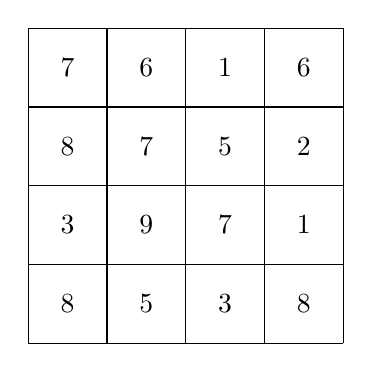
\begin{tikzpicture}[scale=1]
        \draw (0,0) grid (4,4);

        \node[anchor=center] at (0.5, 0.5) {8};
        \node[anchor=center] at (1.5, 0.5) {5};
        \node[anchor=center] at (2.5, 0.5) {3};
        \node[anchor=center] at (3.5, 0.5) {8};

        \node[anchor=center] at (0.5, 1.5) {3};
        \node[anchor=center] at (1.5, 1.5) {9};
        \node[anchor=center] at (2.5, 1.5) {7};
        \node[anchor=center] at (3.5, 1.5) {1};

        \node[anchor=center] at (0.5, 2.5) {8};
        \node[anchor=center] at (1.5, 2.5) {7};
        \node[anchor=center] at (2.5, 2.5) {5};
        \node[anchor=center] at (3.5, 2.5) {2};

        \node[anchor=center] at (0.5, 3.5) {7};
        \node[anchor=center] at (1.5, 3.5) {6};
        \node[anchor=center] at (2.5, 3.5) {1};
        \node[anchor=center] at (3.5, 3.5) {6};
    \end{tikzpicture}
\end{center}
\pagebreak
la suma de cualquier subarreglo se puede calcular con el siguiente árbol
de segmentos:
\begin{center}
    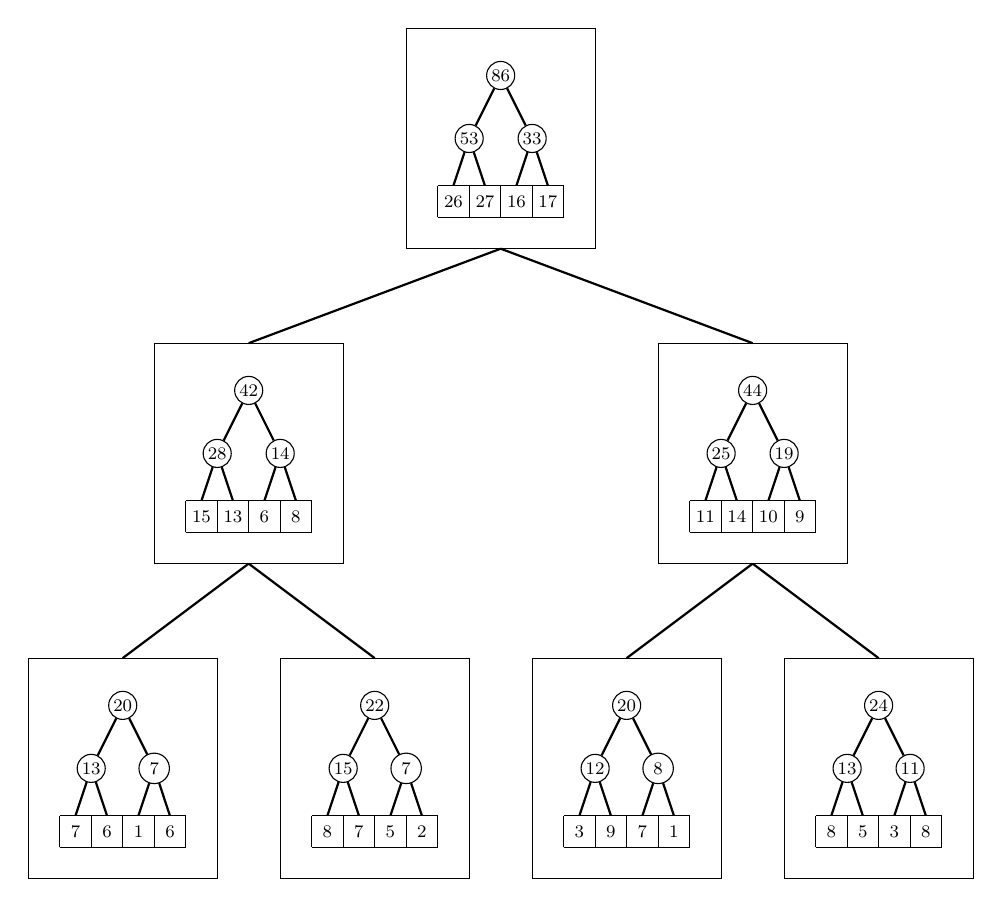
\begin{tikzpicture}[scale=0.4]
        \footnotesize
        \begin{scope}[shift={(-12,0)}]
            \draw (-1,-1) rectangle (5,6);
            \draw (0,0) grid (4,1);
            \node[anchor=center,scale=0.8] at (0.5, 0.5) {7};
            \node[anchor=center,scale=0.8] at (1.5, 0.5) {6};
            \node[anchor=center,scale=0.8] at (2.5, 0.5) {1};
            \node[anchor=center,scale=0.8] at (3.5, 0.5) {6};

            \node[draw, circle,scale=0.8,inner sep=1pt] (a) at (1,2.5) {13};
            \path[draw,thick,-] (a) -- (0.5,1);
            \path[draw,thick,-] (a) -- (1.5,1);
            \node[draw, circle,scale=0.8,inner sep=2.5pt] (b) at (3,2.5) {7};
            \path[draw,thick,-] (b) -- (2.5,1);
            \path[draw,thick,-] (b) -- (3.5,1);

            \node[draw, circle,scale=0.8,inner sep=1pt] (i) at (2,4.5) {20};
            \path[draw,thick,-] (i) -- (a);
            \path[draw,thick,-] (i) -- (b);
        \end{scope}
        \begin{scope}[shift={(-4,0)}]
            \draw (-1,-1) rectangle (5,6);
            \draw (0,0) grid (4,1);
            \node[anchor=center,scale=0.8] at (0.5, 0.5) {8};
            \node[anchor=center,scale=0.8] at (1.5, 0.5) {7};
            \node[anchor=center,scale=0.8] at (2.5, 0.5) {5};
            \node[anchor=center,scale=0.8] at (3.5, 0.5) {2};

            \node[draw, circle,scale=0.8,inner sep=1pt] (a) at (1,2.5) {15};
            \path[draw,thick,-] (a) -- (0.5,1);
            \path[draw,thick,-] (a) -- (1.5,1);
            \node[draw, circle,scale=0.8,inner sep=2.5pt] (b) at (3,2.5) {7};
            \path[draw,thick,-] (b) -- (2.5,1);
            \path[draw,thick,-] (b) -- (3.5,1);

            \node[draw, circle,scale=0.8,inner sep=1pt] (i) at (2,4.5) {22};
            \path[draw,thick,-] (i) -- (a);
            \path[draw,thick,-] (i) -- (b);
        \end{scope}
        \begin{scope}[shift={(4,0)}]
            \draw (-1,-1) rectangle (5,6);
            \draw (0,0) grid (4,1);
            \node[anchor=center,scale=0.8] at (0.5, 0.5) {3};
            \node[anchor=center,scale=0.8] at (1.5, 0.5) {9};
            \node[anchor=center,scale=0.8] at (2.5, 0.5) {7};
            \node[anchor=center,scale=0.8] at (3.5, 0.5) {1};

            \node[draw, circle,scale=0.8,inner sep=1pt] (a) at (1,2.5) {12};
            \path[draw,thick,-] (a) -- (0.5,1);
            \path[draw,thick,-] (a) -- (1.5,1);
            \node[draw, circle,scale=0.8,inner sep=2.5pt] (b) at (3,2.5) {8};
            \path[draw,thick,-] (b) -- (2.5,1);
            \path[draw,thick,-] (b) -- (3.5,1);

            \node[draw, circle,scale=0.8,inner sep=1pt] (i) at (2,4.5) {20};
            \path[draw,thick,-] (i) -- (a);
            \path[draw,thick,-] (i) -- (b);
        \end{scope}
        \begin{scope}[shift={(12,0)}]
            \draw (-1,-1) rectangle (5,6);
            \draw (0,0) grid (4,1);
            \node[anchor=center,scale=0.8] at (0.5, 0.5) {8};
            \node[anchor=center,scale=0.8] at (1.5, 0.5) {5};
            \node[anchor=center,scale=0.8] at (2.5, 0.5) {3};
            \node[anchor=center,scale=0.8] at (3.5, 0.5) {8};

            \node[draw, circle,scale=0.8,inner sep=1pt] (a) at (1,2.5) {13};
            \path[draw,thick,-] (a) -- (0.5,1);
            \path[draw,thick,-] (a) -- (1.5,1);
            \node[draw, circle,scale=0.8,inner sep=1pt] (b) at (3,2.5) {11};
            \path[draw,thick,-] (b) -- (2.5,1);
            \path[draw,thick,-] (b) -- (3.5,1);

            \node[draw, circle,scale=0.8,inner sep=1pt] (i) at (2,4.5) {24};
            \path[draw,thick,-] (i) -- (a);
            \path[draw,thick,-] (i) -- (b);
        \end{scope}
        \begin{scope}[shift={(-8,10)}]
            \draw (-1,-1) rectangle (5,6);
            \draw (0,0) grid (4,1);
            \node[anchor=center,scale=0.8] at (0.5, 0.5) {15};
            \node[anchor=center,scale=0.8] at (1.5, 0.5) {13};
            \node[anchor=center,scale=0.8] at (2.5, 0.5) {6};
            \node[anchor=center,scale=0.8] at (3.5, 0.5) {8};

            \node[draw, circle,scale=0.8,inner sep=1pt] (a) at (1,2.5) {28};
            \path[draw,thick,-] (a) -- (0.5,1);
            \path[draw,thick,-] (a) -- (1.5,1);
            \node[draw, circle,scale=0.8,inner sep=1pt] (b) at (3,2.5) {14};
            \path[draw,thick,-] (b) -- (2.5,1);
            \path[draw,thick,-] (b) -- (3.5,1);

            \node[draw, circle,scale=0.8,inner sep=1pt] (i) at (2,4.5) {42};
            \path[draw,thick,-] (i) -- (a);
            \path[draw,thick,-] (i) -- (b);
        \end{scope}
        \begin{scope}[shift={(8,10)}]
            \draw (-1,-1) rectangle (5,6);
            \draw (0,0) grid (4,1);
            \node[anchor=center,scale=0.8] at (0.5, 0.5) {11};
            \node[anchor=center,scale=0.8] at (1.5, 0.5) {14};
            \node[anchor=center,scale=0.8] at (2.5, 0.5) {10};
            \node[anchor=center,scale=0.8] at (3.5, 0.5) {9};

            \node[draw, circle,scale=0.8,inner sep=1pt] (a) at (1,2.5) {25};
            \path[draw,thick,-] (a) -- (0.5,1);
            \path[draw,thick,-] (a) -- (1.5,1);
            \node[draw, circle,scale=0.8,inner sep=1pt] (b) at (3,2.5) {19};
            \path[draw,thick,-] (b) -- (2.5,1);
            \path[draw,thick,-] (b) -- (3.5,1);

            \node[draw, circle,scale=0.8,inner sep=1pt] (i) at (2,4.5) {44};
            \path[draw,thick,-] (i) -- (a);
            \path[draw,thick,-] (i) -- (b);
        \end{scope}
        \begin{scope}[shift={(0,20)}]
            \draw (-1,-1) rectangle (5,6);
            \draw (0,0) grid (4,1);
            \node[anchor=center,scale=0.8] at (0.5, 0.5) {26};
            \node[anchor=center,scale=0.8] at (1.5, 0.5) {27};
            \node[anchor=center,scale=0.8] at (2.5, 0.5) {16};
            \node[anchor=center,scale=0.8] at (3.5, 0.5) {17};

            \node[draw, circle,scale=0.8,inner sep=1pt] (a) at (1,2.5) {53};
            \path[draw,thick,-] (a) -- (0.5,1);
            \path[draw,thick,-] (a) -- (1.5,1);
            \node[draw, circle,scale=0.8,inner sep=1pt] (b) at (3,2.5) {33};
            \path[draw,thick,-] (b) -- (2.5,1);
            \path[draw,thick,-] (b) -- (3.5,1);

            \node[draw, circle,scale=0.8,inner sep=1pt] (i) at (2,4.5) {86};
            \path[draw,thick,-] (i) -- (a);
            \path[draw,thick,-] (i) -- (b);
        \end{scope}
        \path[draw,thick,-] (2,19) -- (-6,16);
        \path[draw,thick,-] (2,19) -- (10,16);
        \path[draw,thick,-] (-6,9) -- (-10,6);
        \path[draw,thick,-] (-6,9) -- (-2,6);
        \path[draw,thick,-] (10,9) -- (6,6);
        \path[draw,thick,-] (10,9) -- (14,6);
    \end{tikzpicture}
\end{center}

Las operaciones de un árbol de segmentos bidimensional tardan $O(\log^2 n)$,
porque el árbol grande y cada árbol pequeño contiene $O(\log n)$ niveles.
El árbol requiere $O(n^2)$ de memoria, porque cada árbol pequeño contiene
$O(n)$ valores.